\documentclass[a4paper, 12pt]{report}
\usepackage[T2A]{fontenc} 
\usepackage[utf8]{inputenc}
\usepackage[english,russian]{babel} 
\usepackage{amsmath,amsfonts,amssymb,amsthm,mathtools}
\usepackage[left=2cm,right=2cm,top=2cm,bottom=2cm,bindingoffset=0cm]{geometry}
\usepackage{graphicx}
\usepackage[linesnumbered,boxed]{algorithm2e}
\usepackage{verbatim}

\newenvironment{Proof} 
{\par\noindent{$\blacklozenge$}}
{\hfill$\scriptstyle\boxtimes$} 

\newenvironment{example} 
{\par\noindent{\textsc{\textbf{Пример}.}}} 
{\hfill$\scriptstyle\Box$} 

\newtheorem*{theorem}{Теорема} 
\newtheorem*{corollary}{Следствие}
\newtheorem*{lemma}{Лемма}

\newcommand{\RNumb}[1]{\uppercase\expandafter{\romannumeral #1\relax}}
\newcommand{\Rm}{\mathbb{R}}
\newcommand{\Cm}{\mathbb{C}}
\newcommand{\I}{\mathbb{I}}
\newcommand{\N}{\mathbb{N}}
\newcommand{\Z}{\mathbb{Z}}
\newcommand{\Q}{\mathbb{Q}}

\title{\textbf{\Huge{Методы вычислений}}\\Лабораторная работа 1 «Метод Гаусса»\\Выполнила Николаева Ксения, 9 группа}
\date{} 

\begin{document}
    \maketitle

    \textbf{\Huge{Постановка задачи}}\\\\
    Разработать программу на C++, реализующую метод Гаусса с выбором главного элемента по столбцу для решения систем линейных алгебраических уравнений $( Ax = b )$. Использовать тип \textit{double} и выводить предупреждения о невозможности решения при наличии сингулярной матрицы $A$.\\
    Задачи:\\
    1. Решить систему с матрицей $A$ порядка $n = 1000$, заполненной случайными числами от $-100$ до $100$. Вектор точного решения $x$ задать как:
    \[
   x = \begin{pmatrix}
   m \\
   m + 1 \\
   \vdots \\
   m + n - 1
   \end{pmatrix}
   \]
   
   где $m = 8$ — номер студента. Правую часть $b$ вычислить как $b = Ax$.\\ 
   Вывести первые и последние 5 координат векторов $x$ и $ \tilde{x}$ (приближенное решение), а также относительную погрешность и время выполнения.\\
   2. Решить систему с матрицей Гильберта порядка $n = 10$ и $n = m + 30$. Вектор точного решения $x$ задан как:
   \[
   x = \begin{pmatrix}
   1 \\
   2 \\
   \vdots \\
   n
   \end{pmatrix}
   \]
   Правую часть $b$ также вычислить как $b = Ax$.\\
   Вывести векторы$x$ и $\tilde{x}$ (приближенное решение) и относительную погрешность.\\

   \newpage
   \textbf{\Huge{Краткие теоретические сведения}}\\\\
   \textbf{Метод Гаусса используется} для решения систем линейных уравнений, преобразуя систему в верхнюю треугольную форму. При этом выбирается главный элемент (максимальный по модулю) в каждом столбце, что минимизирует ошибки округления и повышает стабильность.\\\\
   \textbf{Псевдокод}

   \begin{algorithm}
       \For{i = 0 ... n - 2} {
       $maxRow = i$\\
       \For{k = i + 1 ... n - 1} {
       if ($|a_{k,i}| > |a_{maxRow,i}|$) $maxRow = k$
       }
       swap ($A_{i}, A_{maxRow}$)\\
       swap ($b_{i}, b_{maxRow}$)\\
       \For{k = i + 1 ... n - 1} {
       $l_{k,i} = \dfrac{a_{k,i}}{a_{i,i}}$\\
       $b_{i} = b_{i} - l_{k,i} \dot b_{i}$\\
       \For{j = i ... n - 1}{
       $a_{k,j} = a_{k,j} - l_{k,i} \dot a_{i,j}$\\
       }
       }
       }
       $x_{n} = \dfrac{b_{n}}{a_{n}}$\\
       \For{i = n - 2 ... 0} {
       $x_{i} = \dfrac{1}{a_{i,i}} (b_{i} - \sum_{j = i + 1}^{n} a_{i,j}x_{j})$\\\\
       }
   \end{algorithm}
   \textbf{Погрешности в вычислениях}делятся на абсолютные и относительные\\
   $\bullet$ Абсолютная погрешность — это разность между истинным и вычисленным значениями\\
   $\bullet$ Относительная погрешность — отношение абсолютной погрешности к истинному значению:$$\delta =  \dfrac {||x - \tilde{x}||_{\infty}}{||x||_{\infty}}$$\\
   Метод Гаусса с выбором главного элемента помогает снизить ошибки округления, улучшая точность вычислений.\\

   \newpage
   \textbf{\Huge{Листинг программы с комментариями}}\\\\
   \begin{verbatim}
#include <bits/stdc++.h>

using namespace std;

const int N = 1e3 + 1;
const int M = 1e3 + 9;

vector<vector<long double>> A;
vector<long double> b;
vector<long double> x;
vector<long double> x1;

int n;
int m = 8;
bool can = 1;

///Создание матрицы для пункта 1
void createMatrix(int n) {
    srand(time(0));
    A.resize(n, vector<long double>(n));
    for (int i = 0; i < n; ++i) {
        for (int j = 0; j < n; ++j) {
            A[i][j] = rand() % 201 - 100;
        }
    }
}
///Создание матрицы для пункта 2
void createHilbertMatrix(int n) {
    A.resize(n, vector<long double>(n));
    for (int i = 0; i < n; ++i) {
        for (int j = 0; j < n; ++j) {
            A[i][j] = 1.0 / (i + j + 1);
        }
    }
}
///Вычисление значений вектора b
void createB(int n) {
    b.resize(n, 0);
    for (int i = 0; i < n; ++i) {
        for (int j = 0; j < n; ++j) {
            b[i] += A[i][j] * x[j];
        }
    }
}
///Метод Гаусса
void GaussianElimination(int n) {
    ///Прямой ход
    for (int i = 0; i < n - 1; ++i) {
        int maxRow = i; ///Столбец с максимальным элементом
        for (int k = i + 1; k < n; ++k) {
            if (fabs(A[k][i]) > fabs(A[maxRow][i])) {
                maxRow = k;
            }
        }

        if (fabs(A[maxRow][i]) < 1e-12) {
            cout << "It is impossible to solve the system:
            the matrix is singular or close to singular in the row " << i + 1 << ".\n";
            can = 0;
            return;
        }
        swap(A[i], A[maxRow]);
        swap(b[i], b[maxRow]);
        for (int k = i + 1; k < n; ++k) {
            long double factor = A[k][i] / A[i][i];
            for (int j = i + 1; j < n; ++j) {
                A[k][j] -= factor * A[i][j];
            }
            b[k] -= factor * b[i];
        }
    }
    ///Обратный ход
    x1.resize(n);
    x1[n - 1] = b[n - 1] / A[n - 1][n - 1];
    for (int i = n - 2; i >= 0; --i) {
        x1[i] = b[i];
        for (int j = i + 1; j < n; ++j) {
            x1[i] -= A[i][j] * x1[j];
        }
        x1[i] /= A[i][i];
    }
}

///Вывод ответа для задачи 1
void printAnswer1(int n) {
    cout << "Exact solution\n";
    for (int i = 0; i < 5; ++i) {
        cout << "x" << i + 1 << " = " << fixed << setprecision(10) << x[i] << '\n';
    }
    cout << "...\n";
    for (int i = n - 5; i < n; ++i) {
        cout << "x" << i + 1 << " = " << fixed << setprecision(10) << x[i] << '\n';
    }
    cout << "---------------------\n";
    cout << "Approximate solution\n";
    for (int i = 0; i < 5; ++i) {
        cout << "~x" << i + 1 << " = " << fixed << setprecision(10) << x1[i] << '\n';
    }
    cout << "...\n";
    for (int i = n - 5; i < n; ++i) {
        cout << "~x" << i + 1 << " = " << fixed << setprecision(10) << x1[i] << '\n';
    }
    cout << "---------------------\n";
    cout << "Relative error\n";
    long double max_diff = 0, max_exact = 0;
    for (int i = 0; i < n; ++i) {
        max_diff = max(max_diff, abs(x[i] - x1[i]));
        max_exact = max(max_exact, abs(x[i]));
    }
    long double relative_error = max_diff / max_exact; ///подсчет
    относительной погрешности
    cout << fixed << setprecision(20) << relative_error << '\n';
}
///Вывод ответа для задачи 2
void printAnswer2(int n) {
    cout << "Exact solution\n";
    for (int i = 0; i < n; ++i) {
        cout << "x" << i + 1 << " = " << fixed << setprecision(10) << x[i] << '\n';
    }
    cout << "---------------------\n";
    cout << "Approximate solution\n";
    for (int i = 0; i < n; ++i) {
        cout << "~x" << i + 1 << " = " << fixed << setprecision(10) << x1[i] << '\n';
    }
    cout << "---------------------\n";
    cout << "Relative error\n";
    long double max_diff = 0, max_exact = 0;
    for (int i = 0; i < n; ++i) {
        max_diff = max(max_diff, abs(x[i] - x1[i]));
        max_exact = max(max_exact, abs(x[i]));
    }
    long double relative_error = max_diff / max_exact; ///подсчет
    относительной погрешности
    cout << fixed << setprecision(20) << relative_error << '\n';
}

int32_t main() {

    freopen("output.txt", "w", stdout);

    ///Решение пункта 1
    cout << "TASK1\n\n";
    n = 1000;
    A.resize(n, vector<long double>(n));
    b.resize(n);
    x.resize(n);

    createMatrix(n);
    for (int i = 0; i < n; ++i) {
        x[i] = m + i;
    }
    createB(n);

    clock_t start = clock();
    GaussianElimination(n);
    clock_t end = clock();
    long double elapsed_time =  double(end - start) / CLOCKS_PER_SEC; ///подсчет затраченного времени

    if (can) {
        printAnswer1(n);
    }
    can = 1;
    cout << "Time: " << elapsed_time << " seconds\n";

    ///Решение пункта 2 с плохо обусловленной матрицей
    cout << "\nTASK2a\n\n";
    n = 10;
    A.clear();
    createHilbertMatrix(n);
    for (int i = 0; i < n; ++i) {
        x[i] = i + 1;
    }
    createB(n);
    GaussianElimination(n);
    if (can) {
        printAnswer2(n);
    }
    can = 1;

    cout << "\nTASK2b\n\n";
    n = m + 30;
    A.clear();
    createHilbertMatrix(n);
    x.resize(n);
    for (int i = 0; i < n; ++i) {
        x[i] = i + 1;
    }
    createB(n);
    GaussianElimination(n);
    if (can) {
        printAnswer2(n);
    }
    return 0;
}
   \end{verbatim}
   \newpage
   \textbf{\Huge{Результаты}}\\\\
   $\bullet$ Результат вычислительного экперимента для задачи 1 с матрицей $A$ порядка $n = 1000$\\
   \begin{center}
        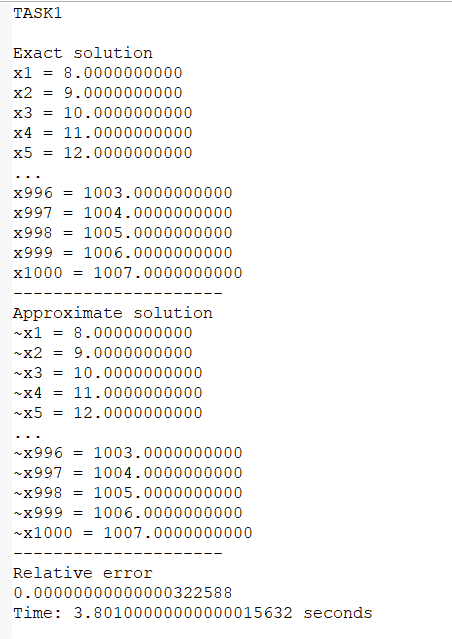
\includegraphics[scale = 0.5]{pic1.png}
   \end{center}
   $\bullet$ Результат вычислительного экперимента для задачи 2 с матрицей $A$ порядка $n = 10$\\
   \begin{center}
       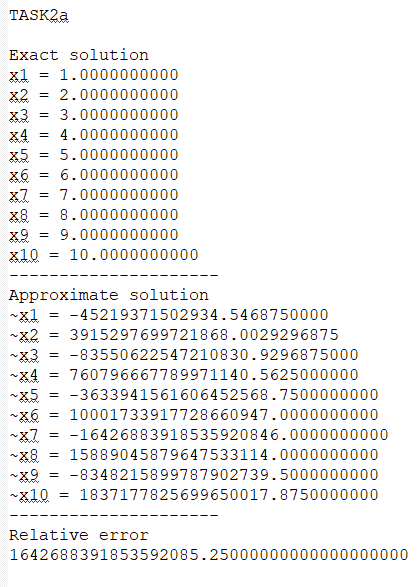
\includegraphics[scale = 0.5]{pic2.png}
   \end{center}
    Из-за того, что матрица плохо обусловленная получилась большая отн. погрешность\\
    $\bullet$ Результат вычислительного экперимента для задачи 2 с матрицей $A$ порядка $n = m + 30$\\
   \begin{center}
       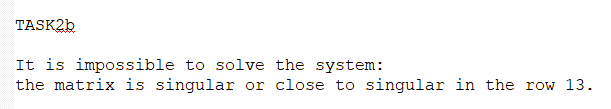
\includegraphics[scale = 0.5]{pic3.png}
   \end{center}
    Из-за того, что матрица плохо обусловленная и имеет большой порядок, в ходе выполнения метода Гаусса получились элементы, близкие к 0, что означает невозможность решения системы\\

    \newpage
   \textbf{\Huge{Выводы}}\\\\
   $\bullet$ Реализация метода Гаусса с выбором главного элемента для численного решения систем линейных алгебраических уравнений показала высокую точность при решении системы с матрицей порядка $n = 1000$, что подтверждается крайне малой относительной погрешностью $0.00000000000000322588$\\
   $\bullet$ Время выполнения программы для матрицы порядка $n = 1000$ составило около $3.8$ секунд, что свидетельствует о приемлемой вычислительной эффективности метода для крупных систем.\\
   $\bullet$ При решении задачи с плохо обусловленной матрицей Гильберта, программа выявила особенности численных методов:для матрицы порядка $n = 10$ была большая относительная погрешность, адля матрицы порядка $n = 38$ система оказалась близка к вырожденной, что потребовало дополнительных проверок и предупреждений о невозможности решения.\\
   
\end{document}


